

\chapter{Хранение и передача данных}

\section{Шина}


\section{RS-триггер}


\section{Регистр}

\begin{center}
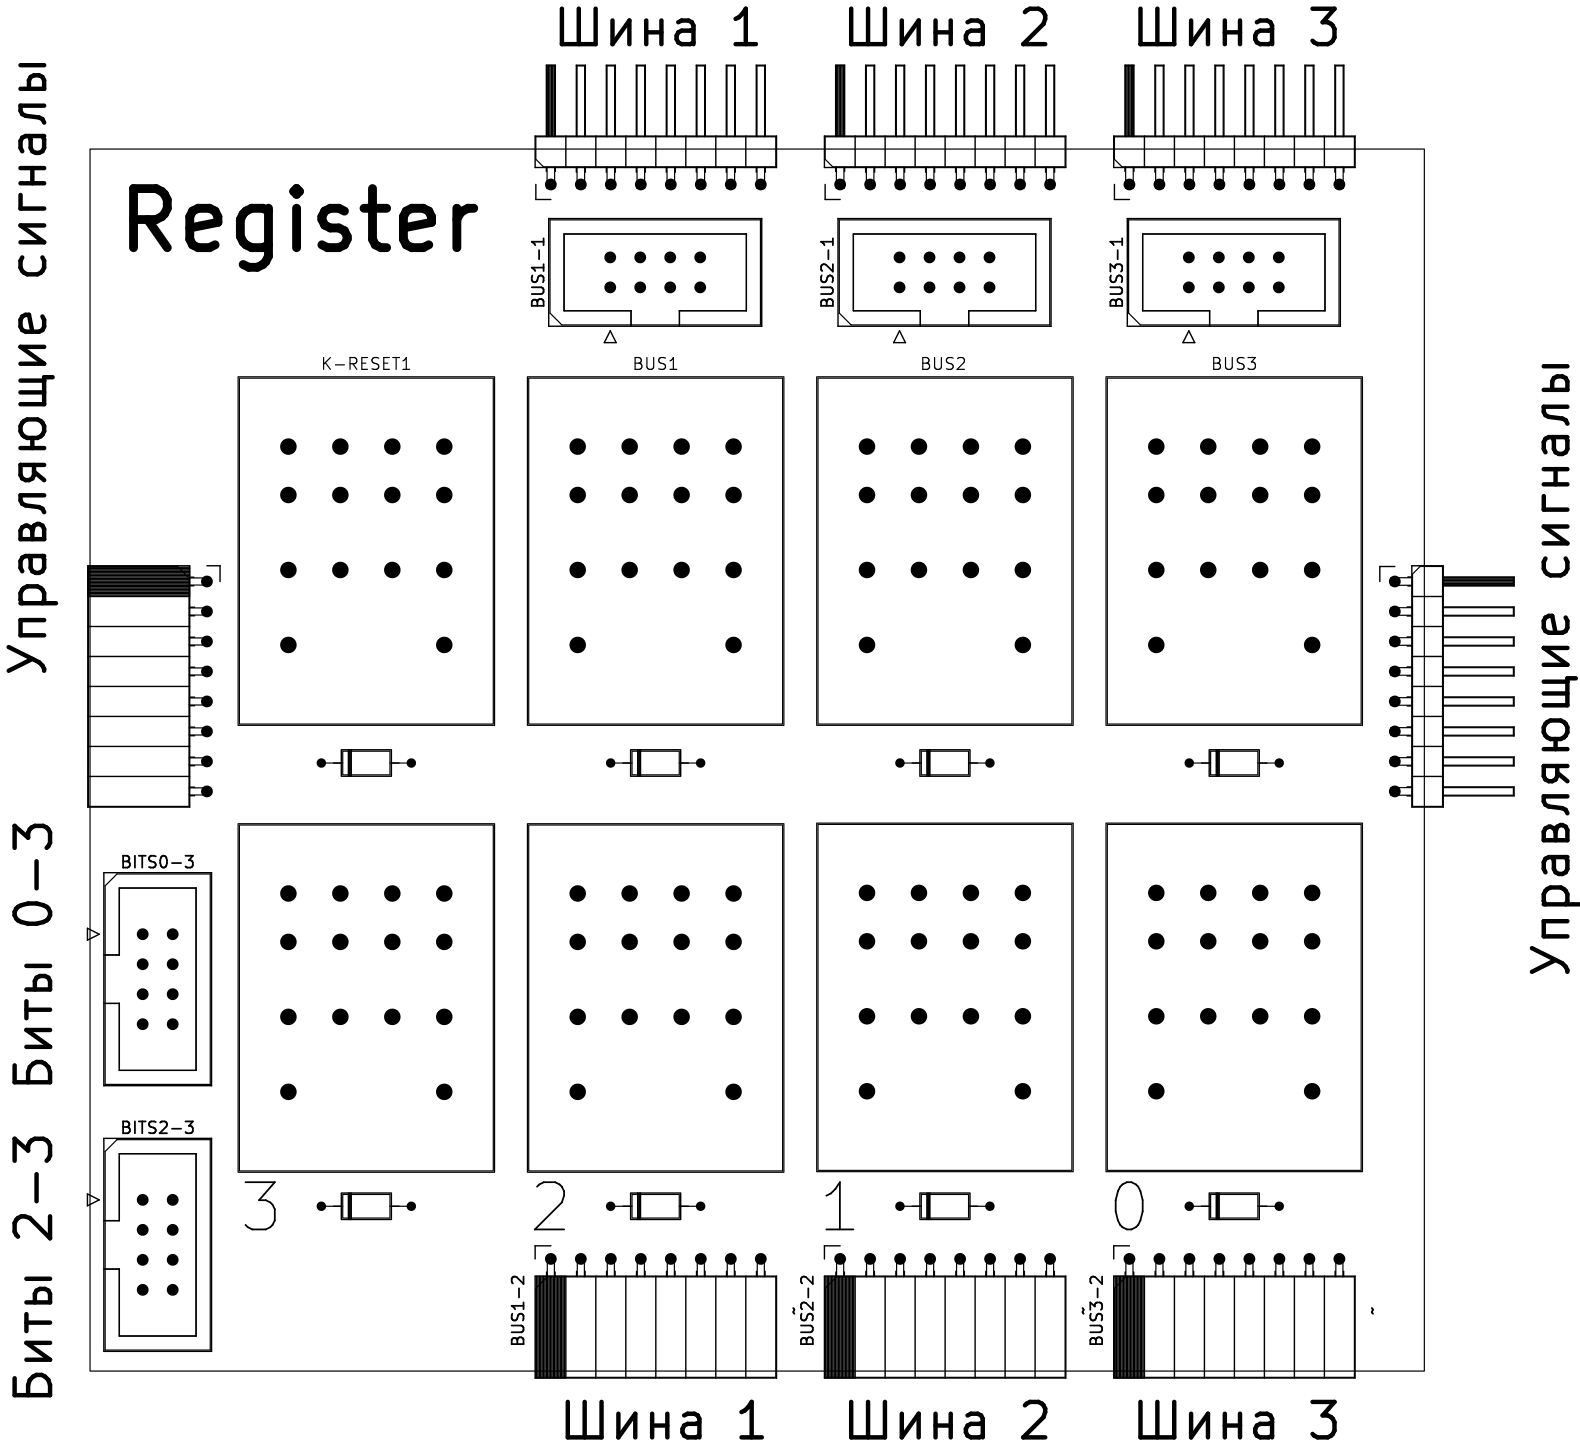
\includegraphics{boards/register.png}
\end{center}

Модуль четырёхбитного регистра состоит из четырёх реле-триггеров,
одного реле для обнуления регистра и трёх реле для подключения
к шинам данных.

Модуль <<Регистр>> имеет следующие разъёмы:
\begin{itemize}
  \item Слева и справа: управляющие сигналы сброса и выборки.
        Можно подключить тумблеры
        для ручного включения сигналов. Также можно соединить несколько
        модулей регистра, чтобы управлять одним набором сигналов сразу
        для $8$, $12$ \ldots бит.
  \item Сверху и снизу: три шины данных. Реле регистра могут
        подключаться к шинам для записи или чтения данных.
  \item Дополнительные разъёмы с битами $0-3$ и $2-3$ для чтения или
        записи значения без подключения к шине.
\end{itemize}

\subsection{Практикум}

Протестировать работу регистра можно собрав следующую схему:

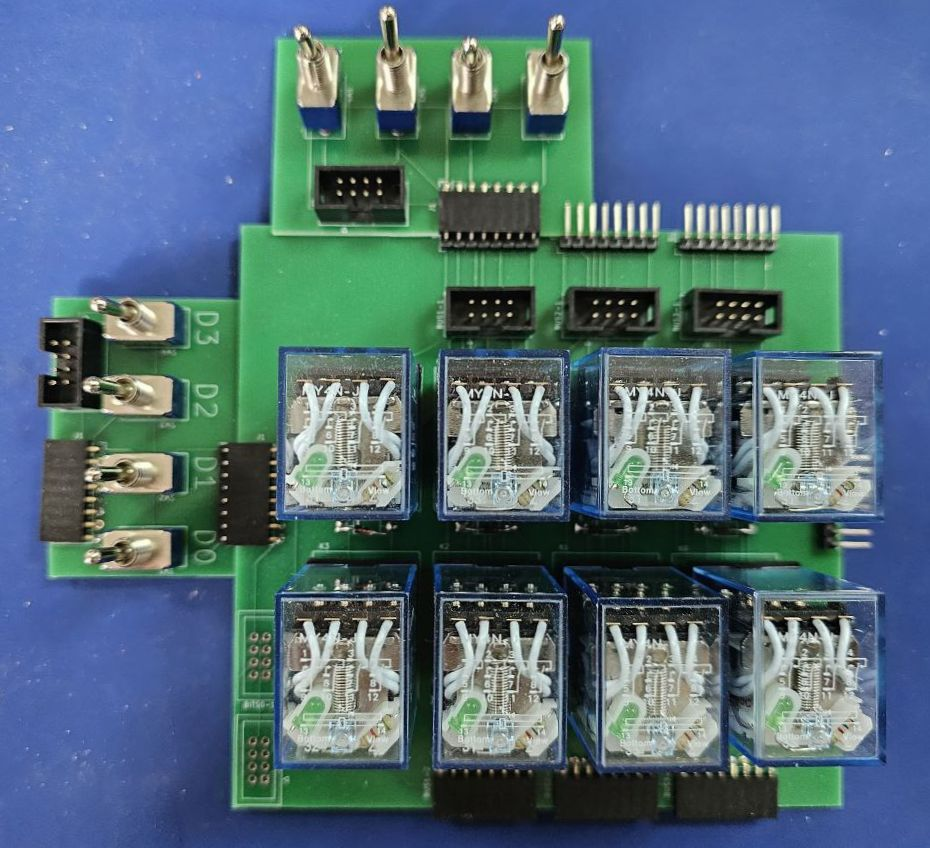
\includegraphics[width=0.5\columnwidth]{photo/register.jpg}

\begin{itemize}
  \item Тумблеры слева управляют работой регистра. Бит 0 --- обнуление, бит 1 --- выборка на шину 1.
  \item Тумблеры сверху нужны для ввода значения регистра. Когда он подключается к шине 1,
        значения, набранное на тумблерах, записывается в регистр.
\end{itemize}

\subsubsection{Регистр без шины}

\begin{enumerate}
    \item Подключить тумблеры проводом к битам $0-3$ вместо шины.
    \item Набирать значение, убедиться, что биты переключаются в $1$, но не возвращаются в $0$.
    \item Обнулить тумблеры с данными.
    \item Включить и выключить сигнал сброса. Убедиться, что значения всех битов теперь $0$.
\end{enumerate}

\subsubsection{Регистр с шиной}

\begin{enumerate}
    \item Отключить все управляющие сигналы.
    \item Набрать значение на тумблерах для данных. Убедиться, что это не влияет на регистр.
    \item Включить и выключить сигнал выборки на шину $1$. Убедиться, что данные записались в регистр.
    \item Включить и выключить сигнал сброса. Убедиться, что значения всех битов теперь $0$.
\end{enumerate}

\subsection{Задачи}

\begin{enumerate}
    \item Придумайте, как скопировать данные из одного регистра в другой, не запоминая их в голове.
\end{enumerate}
